\batchmode
\documentclass[twoside]{book}

% Packages required by doxygen
\usepackage{fixltx2e}
\usepackage{calc}
\usepackage{doxygen}
\usepackage[export]{adjustbox} % also loads graphicx
\usepackage{graphicx}
\usepackage[utf8]{inputenc}
\usepackage{makeidx}
\usepackage{multicol}
\usepackage{multirow}
\PassOptionsToPackage{warn}{textcomp}
\usepackage{textcomp}
\usepackage[nointegrals]{wasysym}
\usepackage[table]{xcolor}

% Font selection
\usepackage[T1]{fontenc}
\usepackage[scaled=.90]{helvet}
\usepackage{courier}
\usepackage{amssymb}
\usepackage{sectsty}
\renewcommand{\familydefault}{\sfdefault}
\allsectionsfont{%
  \fontseries{bc}\selectfont%
  \color{darkgray}%
}
\renewcommand{\DoxyLabelFont}{%
  \fontseries{bc}\selectfont%
  \color{darkgray}%
}
\newcommand{\+}{\discretionary{\mbox{\scriptsize$\hookleftarrow$}}{}{}}

% Page & text layout
\usepackage{geometry}
\geometry{%
  a4paper,%
  top=2.5cm,%
  bottom=2.5cm,%
  left=2.5cm,%
  right=2.5cm%
}
\tolerance=750
\hfuzz=15pt
\hbadness=750
\setlength{\emergencystretch}{15pt}
\setlength{\parindent}{0cm}
\setlength{\parskip}{3ex plus 2ex minus 2ex}
\makeatletter
\renewcommand{\paragraph}{%
  \@startsection{paragraph}{4}{0ex}{-1.0ex}{1.0ex}{%
    \normalfont\normalsize\bfseries\SS@parafont%
  }%
}
\renewcommand{\subparagraph}{%
  \@startsection{subparagraph}{5}{0ex}{-1.0ex}{1.0ex}{%
    \normalfont\normalsize\bfseries\SS@subparafont%
  }%
}
\makeatother

% Headers & footers
\usepackage{fancyhdr}
\pagestyle{fancyplain}
\fancyhead[LE]{\fancyplain{}{\bfseries\thepage}}
\fancyhead[CE]{\fancyplain{}{}}
\fancyhead[RE]{\fancyplain{}{\bfseries\leftmark}}
\fancyhead[LO]{\fancyplain{}{\bfseries\rightmark}}
\fancyhead[CO]{\fancyplain{}{}}
\fancyhead[RO]{\fancyplain{}{\bfseries\thepage}}
\fancyfoot[LE]{\fancyplain{}{}}
\fancyfoot[CE]{\fancyplain{}{}}
\fancyfoot[RE]{\fancyplain{}{\bfseries\scriptsize Generated by Doxygen }}
\fancyfoot[LO]{\fancyplain{}{\bfseries\scriptsize Generated by Doxygen }}
\fancyfoot[CO]{\fancyplain{}{}}
\fancyfoot[RO]{\fancyplain{}{}}
\renewcommand{\footrulewidth}{0.4pt}
\renewcommand{\chaptermark}[1]{%
  \markboth{#1}{}%
}
\renewcommand{\sectionmark}[1]{%
  \markright{\thesection\ #1}%
}

% Indices & bibliography
\usepackage{natbib}
\usepackage[titles]{tocloft}
\setcounter{tocdepth}{3}
\setcounter{secnumdepth}{5}
\makeindex

% Hyperlinks (required, but should be loaded last)
\usepackage{ifpdf}
\ifpdf
  \usepackage[pdftex,pagebackref=true]{hyperref}
\else
  \usepackage[ps2pdf,pagebackref=true]{hyperref}
\fi
\hypersetup{%
  colorlinks=true,%
  linkcolor=blue,%
  citecolor=blue,%
  unicode%
}

% Custom commands
\newcommand{\clearemptydoublepage}{%
  \newpage{\pagestyle{empty}\cleardoublepage}%
}

\usepackage{caption}
\captionsetup{labelsep=space,justification=centering,font={bf},singlelinecheck=off,skip=4pt,position=top}

%===== C O N T E N T S =====

\begin{document}

% Titlepage & ToC
\hypersetup{pageanchor=false,
             bookmarksnumbered=true
            }
\pagenumbering{alph}
\pagenumbering{arabic}
\hypersetup{pageanchor=true}

%--- Begin generated contents ---
\chapter{Demo problem\+: A one-\/dimensional Poisson problem}
\label{index}\hypertarget{index}{}\hypertarget{index_q}{}\section{A few quick questions...}\label{index_q}
Since {\ttfamily oomph-\/lib} is developed as open-\/source software, any evidence that the code is being downloaded and used is very helpful for us as it helps to justify our continued work on this project.

We would therefore be extremely grateful if you could provide the information requested in the form below. Pressing the \char`\"{}submit\char`\"{} button will get you to the actual download page.

{\bfseries Note\+:} 
\begin{DoxyItemize}
\item All information will be treated as confidential. 
\item If you provide your email address and check the appropriate box we will add you to our mailing list to inform you of upgrades and bug fixes to the code. Rest assured that the mailing list is {\bfseries very low volume} -- we have better things to do than to bombard you with email. 
\item If you still feel reluctant to provide any of the information requested, feel free to enter some dummy input. The form will check that {\bfseries some} information has been entered but entering your name as \char`\"{}\+Joe Cool\char`\"{} is perfectly acceptable -- this is to discourage people from not providing the information simply because they are too lazy to type... 
\end{DoxyItemize}



 







 

 \hypertarget{index_pdf}{}\section{P\+D\+F file}\label{index_pdf}
A \href{../latex/refman.pdf}{\tt pdf version} of this document is available. \end{document}

\chapter{Namespace Index}
\section{Namespace List}
Here is a list of all namespaces with brief descriptions\+:\begin{DoxyCompactList}
\item\contentsline{section}{\hyperlink{namespaceGlobal__Physical__Variables}{Global\+\_\+\+Physical\+\_\+\+Variables} \\*Global variables that represent physical properties }{\pageref{namespaceGlobal__Physical__Variables}}{}
\item\contentsline{section}{\hyperlink{namespaceoomph}{oomph} }{\pageref{namespaceoomph}}{}
\item\contentsline{section}{\hyperlink{namespacePhysical__Variables}{Physical\+\_\+\+Variables} \\*Namespace for the solution of 2D linear shell equation }{\pageref{namespacePhysical__Variables}}{}
\end{DoxyCompactList}

\chapter{Hierarchical Index}
\section{Class Hierarchy}
This inheritance list is sorted roughly, but not completely, alphabetically\+:\begin{DoxyCompactList}
\item Problem\begin{DoxyCompactList}
\item \contentsline{section}{Unstructured\+Solid\+Problem$<$ E\+L\+E\+M\+E\+NT $>$}{\pageref{classUnstructuredSolidProblem}}{}
\end{DoxyCompactList}
\end{DoxyCompactList}

\chapter{Class Index}
\section{Class List}
Here are the classes, structs, unions and interfaces with brief descriptions\+:\begin{DoxyCompactList}
\item\contentsline{section}{\hyperlink{classPMLProblem}{P\+M\+L\+Problem$<$ E\+L\+E\+M\+E\+N\+T $>$} }{\pageref{classPMLProblem}}{}
\item\contentsline{section}{\hyperlink{classGlobalParameters_1_1TestPMLMapping}{Global\+Parameters\+::\+Test\+P\+M\+L\+Mapping} }{\pageref{classGlobalParameters_1_1TestPMLMapping}}{}
\end{DoxyCompactList}

\chapter{File Index}
\section{File List}
Here is a list of all files with brief descriptions\+:\begin{DoxyCompactList}
\item\contentsline{section}{\hyperlink{jeffery__orbit_8cc}{jeffery\+\_\+orbit.\+cc} }{\pageref{jeffery__orbit_8cc}}{}
\item\contentsline{section}{\hyperlink{jeffery__orbit_8txt__doxygenified_8h}{jeffery\+\_\+orbit.\+txt\+\_\+doxygenified.\+h} }{\pageref{jeffery__orbit_8txt__doxygenified_8h}}{}
\item\contentsline{section}{\hyperlink{my__taylor__hood__elements_8h}{my\+\_\+taylor\+\_\+hood\+\_\+elements.\+h} }{\pageref{my__taylor__hood__elements_8h}}{}
\end{DoxyCompactList}

\chapter{Namespace Documentation}
\hypertarget{namespaceFishSolnOneDPoisson}{}\section{Fish\+Soln\+One\+D\+Poisson Namespace Reference}
\label{namespaceFishSolnOneDPoisson}\index{Fish\+Soln\+One\+D\+Poisson@{Fish\+Soln\+One\+D\+Poisson}}


Namespace for fish-\/shaped solution of 1D Poisson equation.  


\subsection*{Functions}
\begin{DoxyCompactItemize}
\item 
void \hyperlink{namespaceFishSolnOneDPoisson_a52c9346f567cb68fe20268a592deb4bc}{get\+\_\+exact\+\_\+u} (const Vector$<$ double $>$ \&x, Vector$<$ double $>$ \&u)
\begin{DoxyCompactList}\small\item\em Exact, fish-\/shaped solution as a 1D vector. \end{DoxyCompactList}\item 
void \hyperlink{namespaceFishSolnOneDPoisson_afd2f5aef6b8868526dbf8e74d379697f}{source\+\_\+function} (const Vector$<$ double $>$ \&x, double \&source)
\begin{DoxyCompactList}\small\item\em Source function required to make the fish shape an exact solution. \end{DoxyCompactList}\end{DoxyCompactItemize}
\subsection*{Variables}
\begin{DoxyCompactItemize}
\item 
int \hyperlink{namespaceFishSolnOneDPoisson_a108e814ef887ffcc8caa7c65a7d30f06}{Sign} =-\/1
\begin{DoxyCompactList}\small\item\em Sign of the source function (-\/ gives the upper half of the fish, + the lower half) \end{DoxyCompactList}\end{DoxyCompactItemize}


\subsection{Detailed Description}
Namespace for fish-\/shaped solution of 1D Poisson equation. 

\subsection{Function Documentation}
\mbox{\Hypertarget{namespaceFishSolnOneDPoisson_a52c9346f567cb68fe20268a592deb4bc}\label{namespaceFishSolnOneDPoisson_a52c9346f567cb68fe20268a592deb4bc}} 
\index{Fish\+Soln\+One\+D\+Poisson@{Fish\+Soln\+One\+D\+Poisson}!get\+\_\+exact\+\_\+u@{get\+\_\+exact\+\_\+u}}
\index{get\+\_\+exact\+\_\+u@{get\+\_\+exact\+\_\+u}!Fish\+Soln\+One\+D\+Poisson@{Fish\+Soln\+One\+D\+Poisson}}
\subsubsection{\texorpdfstring{get\+\_\+exact\+\_\+u()}{get\_exact\_u()}}
{\footnotesize\ttfamily void Fish\+Soln\+One\+D\+Poisson\+::get\+\_\+exact\+\_\+u (\begin{DoxyParamCaption}\item[{const Vector$<$ double $>$ \&}]{x,  }\item[{Vector$<$ double $>$ \&}]{u }\end{DoxyParamCaption})}



Exact, fish-\/shaped solution as a 1D vector. 



Definition at line 58 of file one\+\_\+d\+\_\+poisson.\+cc.



Referenced by One\+D\+Poisson\+Problem$<$ E\+L\+E\+M\+E\+N\+T $>$\+::actions\+\_\+before\+\_\+newton\+\_\+solve(), and One\+D\+Poisson\+Problem$<$ E\+L\+E\+M\+E\+N\+T $>$\+::doc\+\_\+solution().

\mbox{\Hypertarget{namespaceFishSolnOneDPoisson_afd2f5aef6b8868526dbf8e74d379697f}\label{namespaceFishSolnOneDPoisson_afd2f5aef6b8868526dbf8e74d379697f}} 
\index{Fish\+Soln\+One\+D\+Poisson@{Fish\+Soln\+One\+D\+Poisson}!source\+\_\+function@{source\+\_\+function}}
\index{source\+\_\+function@{source\+\_\+function}!Fish\+Soln\+One\+D\+Poisson@{Fish\+Soln\+One\+D\+Poisson}}
\subsubsection{\texorpdfstring{source\+\_\+function()}{source\_function()}}
{\footnotesize\ttfamily void Fish\+Soln\+One\+D\+Poisson\+::source\+\_\+function (\begin{DoxyParamCaption}\item[{const Vector$<$ double $>$ \&}]{x,  }\item[{double \&}]{source }\end{DoxyParamCaption})}



Source function required to make the fish shape an exact solution. 



Definition at line 65 of file one\+\_\+d\+\_\+poisson.\+cc.



Referenced by main().



\subsection{Variable Documentation}
\mbox{\Hypertarget{namespaceFishSolnOneDPoisson_a108e814ef887ffcc8caa7c65a7d30f06}\label{namespaceFishSolnOneDPoisson_a108e814ef887ffcc8caa7c65a7d30f06}} 
\index{Fish\+Soln\+One\+D\+Poisson@{Fish\+Soln\+One\+D\+Poisson}!Sign@{Sign}}
\index{Sign@{Sign}!Fish\+Soln\+One\+D\+Poisson@{Fish\+Soln\+One\+D\+Poisson}}
\subsubsection{\texorpdfstring{Sign}{Sign}}
{\footnotesize\ttfamily int Fish\+Soln\+One\+D\+Poisson\+::\+Sign =-\/1}



Sign of the source function (-\/ gives the upper half of the fish, + the lower half) 



Definition at line 54 of file one\+\_\+d\+\_\+poisson.\+cc.



Referenced by main().


\chapter{Class Documentation}
\hypertarget{classOneDPoissonProblem}{}\section{One\+D\+Poisson\+Problem$<$ E\+L\+E\+M\+E\+NT $>$ Class Template Reference}
\label{classOneDPoissonProblem}\index{One\+D\+Poisson\+Problem$<$ E\+L\+E\+M\+E\+N\+T $>$@{One\+D\+Poisson\+Problem$<$ E\+L\+E\+M\+E\+N\+T $>$}}


1D Poisson problem in unit interval.  


Inheritance diagram for One\+D\+Poisson\+Problem$<$ E\+L\+E\+M\+E\+NT $>$\+:\begin{figure}[H]
\begin{center}
\leavevmode
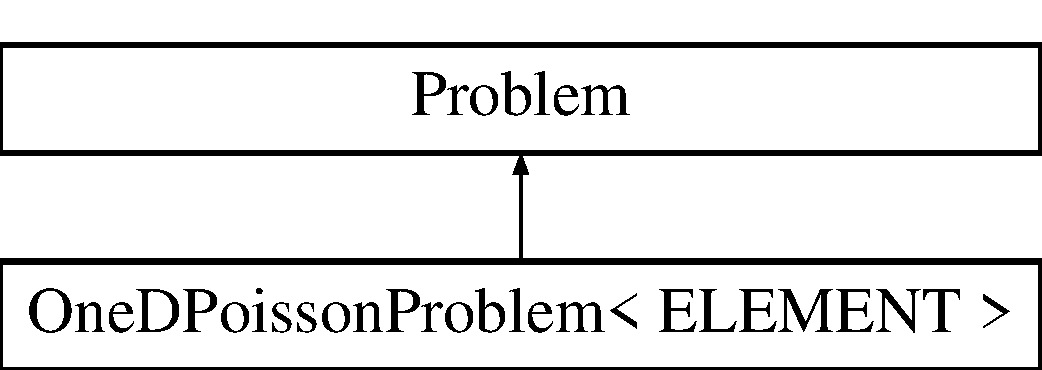
\includegraphics[height=2.000000cm]{classOneDPoissonProblem}
\end{center}
\end{figure}
\subsection*{Public Member Functions}
\begin{DoxyCompactItemize}
\item 
\hyperlink{classOneDPoissonProblem_ab814af5dfd3b7ae665cd20e27da5d9ae}{One\+D\+Poisson\+Problem} (const unsigned \&n\+\_\+element, Poisson\+Equations$<$ 1 $>$\+::Poisson\+Source\+Fct\+Pt source\+\_\+fct\+\_\+pt)
\begin{DoxyCompactList}\small\item\em Constructor\+: Pass number of elements and pointer to source function. \end{DoxyCompactList}\item 
\hyperlink{classOneDPoissonProblem_a940fa32d7939788e27b708818fb046ec}{$\sim$\+One\+D\+Poisson\+Problem} ()
\begin{DoxyCompactList}\small\item\em Destructor (empty) \end{DoxyCompactList}\item 
void \hyperlink{classOneDPoissonProblem_a6e42423869771fbd216326cba516a76b}{actions\+\_\+before\+\_\+newton\+\_\+solve} ()
\begin{DoxyCompactList}\small\item\em Update the problem specs before solve\+: (Re)set boundary conditions. \end{DoxyCompactList}\item 
void \hyperlink{classOneDPoissonProblem_ab023d367cc68b77a7828536333c924ed}{actions\+\_\+after\+\_\+newton\+\_\+solve} ()
\begin{DoxyCompactList}\small\item\em Update the problem specs after solve (empty) \end{DoxyCompactList}\item 
void \hyperlink{classOneDPoissonProblem_aaf42d034e42e7615acfa262a9c56b638}{doc\+\_\+solution} (const unsigned \&label)
\begin{DoxyCompactList}\small\item\em Doc the solution, pass the number of the case considered, so that output files can be distinguished. \end{DoxyCompactList}\end{DoxyCompactItemize}
\subsection*{Private Attributes}
\begin{DoxyCompactItemize}
\item 
Poisson\+Equations$<$ 1 $>$\+::Poisson\+Source\+Fct\+Pt \hyperlink{classOneDPoissonProblem_a5fdff4b9218f56dec7fbc282f2428eef}{Source\+\_\+fct\+\_\+pt}
\begin{DoxyCompactList}\small\item\em Pointer to source function. \end{DoxyCompactList}\end{DoxyCompactItemize}


\subsection{Detailed Description}
\subsubsection*{template$<$class E\+L\+E\+M\+E\+NT$>$\newline
class One\+D\+Poisson\+Problem$<$ E\+L\+E\+M\+E\+N\+T $>$}

1D Poisson problem in unit interval. 

Definition at line 82 of file one\+\_\+d\+\_\+poisson.\+cc.



\subsection{Constructor \& Destructor Documentation}
\mbox{\Hypertarget{classOneDPoissonProblem_ab814af5dfd3b7ae665cd20e27da5d9ae}\label{classOneDPoissonProblem_ab814af5dfd3b7ae665cd20e27da5d9ae}} 
\index{One\+D\+Poisson\+Problem@{One\+D\+Poisson\+Problem}!One\+D\+Poisson\+Problem@{One\+D\+Poisson\+Problem}}
\index{One\+D\+Poisson\+Problem@{One\+D\+Poisson\+Problem}!One\+D\+Poisson\+Problem@{One\+D\+Poisson\+Problem}}
\subsubsection{\texorpdfstring{One\+D\+Poisson\+Problem()}{OneDPoissonProblem()}}
{\footnotesize\ttfamily template$<$class E\+L\+E\+M\+E\+NT $>$ \\
\hyperlink{classOneDPoissonProblem}{One\+D\+Poisson\+Problem}$<$ E\+L\+E\+M\+E\+NT $>$\+::\hyperlink{classOneDPoissonProblem}{One\+D\+Poisson\+Problem} (\begin{DoxyParamCaption}\item[{const unsigned \&}]{n\+\_\+element,  }\item[{Poisson\+Equations$<$ 1 $>$\+::Poisson\+Source\+Fct\+Pt}]{source\+\_\+fct\+\_\+pt }\end{DoxyParamCaption})}



Constructor\+: Pass number of elements and pointer to source function. 

Constructor for 1D Poisson problem in unit interval. Discretise the 1D domain with n\+\_\+element elements of type E\+L\+E\+M\+E\+NT. Specify function pointer to source function. 

Definition at line 124 of file one\+\_\+d\+\_\+poisson.\+cc.



References One\+D\+Poisson\+Problem$<$ E\+L\+E\+M\+E\+N\+T $>$\+::\+Source\+\_\+fct\+\_\+pt.

\mbox{\Hypertarget{classOneDPoissonProblem_a940fa32d7939788e27b708818fb046ec}\label{classOneDPoissonProblem_a940fa32d7939788e27b708818fb046ec}} 
\index{One\+D\+Poisson\+Problem@{One\+D\+Poisson\+Problem}!````~One\+D\+Poisson\+Problem@{$\sim$\+One\+D\+Poisson\+Problem}}
\index{````~One\+D\+Poisson\+Problem@{$\sim$\+One\+D\+Poisson\+Problem}!One\+D\+Poisson\+Problem@{One\+D\+Poisson\+Problem}}
\subsubsection{\texorpdfstring{$\sim$\+One\+D\+Poisson\+Problem()}{~OneDPoissonProblem()}}
{\footnotesize\ttfamily template$<$class E\+L\+E\+M\+E\+NT$>$ \\
\hyperlink{classOneDPoissonProblem}{One\+D\+Poisson\+Problem}$<$ E\+L\+E\+M\+E\+NT $>$\+::$\sim$\hyperlink{classOneDPoissonProblem}{One\+D\+Poisson\+Problem} (\begin{DoxyParamCaption}{ }\end{DoxyParamCaption})\hspace{0.3cm}{\ttfamily [inline]}}



Destructor (empty) 



Definition at line 92 of file one\+\_\+d\+\_\+poisson.\+cc.



\subsection{Member Function Documentation}
\mbox{\Hypertarget{classOneDPoissonProblem_ab023d367cc68b77a7828536333c924ed}\label{classOneDPoissonProblem_ab023d367cc68b77a7828536333c924ed}} 
\index{One\+D\+Poisson\+Problem@{One\+D\+Poisson\+Problem}!actions\+\_\+after\+\_\+newton\+\_\+solve@{actions\+\_\+after\+\_\+newton\+\_\+solve}}
\index{actions\+\_\+after\+\_\+newton\+\_\+solve@{actions\+\_\+after\+\_\+newton\+\_\+solve}!One\+D\+Poisson\+Problem@{One\+D\+Poisson\+Problem}}
\subsubsection{\texorpdfstring{actions\+\_\+after\+\_\+newton\+\_\+solve()}{actions\_after\_newton\_solve()}}
{\footnotesize\ttfamily template$<$class E\+L\+E\+M\+E\+NT$>$ \\
void \hyperlink{classOneDPoissonProblem}{One\+D\+Poisson\+Problem}$<$ E\+L\+E\+M\+E\+NT $>$\+::actions\+\_\+after\+\_\+newton\+\_\+solve (\begin{DoxyParamCaption}{ }\end{DoxyParamCaption})\hspace{0.3cm}{\ttfamily [inline]}}



Update the problem specs after solve (empty) 



Definition at line 101 of file one\+\_\+d\+\_\+poisson.\+cc.

\mbox{\Hypertarget{classOneDPoissonProblem_a6e42423869771fbd216326cba516a76b}\label{classOneDPoissonProblem_a6e42423869771fbd216326cba516a76b}} 
\index{One\+D\+Poisson\+Problem@{One\+D\+Poisson\+Problem}!actions\+\_\+before\+\_\+newton\+\_\+solve@{actions\+\_\+before\+\_\+newton\+\_\+solve}}
\index{actions\+\_\+before\+\_\+newton\+\_\+solve@{actions\+\_\+before\+\_\+newton\+\_\+solve}!One\+D\+Poisson\+Problem@{One\+D\+Poisson\+Problem}}
\subsubsection{\texorpdfstring{actions\+\_\+before\+\_\+newton\+\_\+solve()}{actions\_before\_newton\_solve()}}
{\footnotesize\ttfamily template$<$class E\+L\+E\+M\+E\+NT $>$ \\
void \hyperlink{classOneDPoissonProblem}{One\+D\+Poisson\+Problem}$<$ E\+L\+E\+M\+E\+NT $>$\+::actions\+\_\+before\+\_\+newton\+\_\+solve (\begin{DoxyParamCaption}{ }\end{DoxyParamCaption})}



Update the problem specs before solve\+: (Re)set boundary conditions. 

Update the problem specs before solve\+: (Re)set boundary values from the exact solution. 

Definition at line 174 of file one\+\_\+d\+\_\+poisson.\+cc.



References Fish\+Soln\+One\+D\+Poisson\+::get\+\_\+exact\+\_\+u().

\mbox{\Hypertarget{classOneDPoissonProblem_aaf42d034e42e7615acfa262a9c56b638}\label{classOneDPoissonProblem_aaf42d034e42e7615acfa262a9c56b638}} 
\index{One\+D\+Poisson\+Problem@{One\+D\+Poisson\+Problem}!doc\+\_\+solution@{doc\+\_\+solution}}
\index{doc\+\_\+solution@{doc\+\_\+solution}!One\+D\+Poisson\+Problem@{One\+D\+Poisson\+Problem}}
\subsubsection{\texorpdfstring{doc\+\_\+solution()}{doc\_solution()}}
{\footnotesize\ttfamily template$<$class E\+L\+E\+M\+E\+NT $>$ \\
void \hyperlink{classOneDPoissonProblem}{One\+D\+Poisson\+Problem}$<$ E\+L\+E\+M\+E\+NT $>$\+::doc\+\_\+solution (\begin{DoxyParamCaption}\item[{const unsigned \&}]{label }\end{DoxyParamCaption})}



Doc the solution, pass the number of the case considered, so that output files can be distinguished. 

Doc the solution in tecplot format. Label files with label. 

Definition at line 220 of file one\+\_\+d\+\_\+poisson.\+cc.



References Fish\+Soln\+One\+D\+Poisson\+::get\+\_\+exact\+\_\+u().



Referenced by main().



\subsection{Member Data Documentation}
\mbox{\Hypertarget{classOneDPoissonProblem_a5fdff4b9218f56dec7fbc282f2428eef}\label{classOneDPoissonProblem_a5fdff4b9218f56dec7fbc282f2428eef}} 
\index{One\+D\+Poisson\+Problem@{One\+D\+Poisson\+Problem}!Source\+\_\+fct\+\_\+pt@{Source\+\_\+fct\+\_\+pt}}
\index{Source\+\_\+fct\+\_\+pt@{Source\+\_\+fct\+\_\+pt}!One\+D\+Poisson\+Problem@{One\+D\+Poisson\+Problem}}
\subsubsection{\texorpdfstring{Source\+\_\+fct\+\_\+pt}{Source\_fct\_pt}}
{\footnotesize\ttfamily template$<$class E\+L\+E\+M\+E\+NT$>$ \\
Poisson\+Equations$<$1$>$\+::Poisson\+Source\+Fct\+Pt \hyperlink{classOneDPoissonProblem}{One\+D\+Poisson\+Problem}$<$ E\+L\+E\+M\+E\+NT $>$\+::Source\+\_\+fct\+\_\+pt\hspace{0.3cm}{\ttfamily [private]}}



Pointer to source function. 



Definition at line 110 of file one\+\_\+d\+\_\+poisson.\+cc.



Referenced by One\+D\+Poisson\+Problem$<$ E\+L\+E\+M\+E\+N\+T $>$\+::\+One\+D\+Poisson\+Problem().



The documentation for this class was generated from the following file\+:\begin{DoxyCompactItemize}
\item 
\hyperlink{one__d__poisson_8cc}{one\+\_\+d\+\_\+poisson.\+cc}\end{DoxyCompactItemize}

\chapter{File Documentation}
\hypertarget{one__d__poisson_8cc}{}\section{one\+\_\+d\+\_\+poisson.\+cc File Reference}
\label{one__d__poisson_8cc}\index{one\+\_\+d\+\_\+poisson.\+cc@{one\+\_\+d\+\_\+poisson.\+cc}}
\subsection*{Classes}
\begin{DoxyCompactItemize}
\item 
class \hyperlink{classOneDPoissonProblem}{One\+D\+Poisson\+Problem$<$ E\+L\+E\+M\+E\+N\+T $>$}
\begin{DoxyCompactList}\small\item\em 1D Poisson problem in unit interval. \end{DoxyCompactList}\end{DoxyCompactItemize}
\subsection*{Namespaces}
\begin{DoxyCompactItemize}
\item 
 \hyperlink{namespaceFishSolnOneDPoisson}{Fish\+Soln\+One\+D\+Poisson}
\begin{DoxyCompactList}\small\item\em Namespace for fish-\/shaped solution of 1D Poisson equation. \end{DoxyCompactList}\end{DoxyCompactItemize}
\subsection*{Functions}
\begin{DoxyCompactItemize}
\item 
void \hyperlink{namespaceFishSolnOneDPoisson_a52c9346f567cb68fe20268a592deb4bc}{Fish\+Soln\+One\+D\+Poisson\+::get\+\_\+exact\+\_\+u} (const Vector$<$ double $>$ \&x, Vector$<$ double $>$ \&u)
\begin{DoxyCompactList}\small\item\em Exact, fish-\/shaped solution as a 1D vector. \end{DoxyCompactList}\item 
void \hyperlink{namespaceFishSolnOneDPoisson_afd2f5aef6b8868526dbf8e74d379697f}{Fish\+Soln\+One\+D\+Poisson\+::source\+\_\+function} (const Vector$<$ double $>$ \&x, double \&source)
\begin{DoxyCompactList}\small\item\em Source function required to make the fish shape an exact solution. \end{DoxyCompactList}\item 
int \hyperlink{one__d__poisson_8cc_ae66f6b31b5ad750f1fe042a706a4e3d4}{main} ()
\begin{DoxyCompactList}\small\item\em Driver for 1D Poisson problem. \end{DoxyCompactList}\end{DoxyCompactItemize}
\subsection*{Variables}
\begin{DoxyCompactItemize}
\item 
int \hyperlink{namespaceFishSolnOneDPoisson_a108e814ef887ffcc8caa7c65a7d30f06}{Fish\+Soln\+One\+D\+Poisson\+::\+Sign} =-\/1
\begin{DoxyCompactList}\small\item\em Sign of the source function (-\/ gives the upper half of the fish, + the lower half) \end{DoxyCompactList}\end{DoxyCompactItemize}


\subsection{Function Documentation}
\mbox{\Hypertarget{one__d__poisson_8cc_ae66f6b31b5ad750f1fe042a706a4e3d4}\label{one__d__poisson_8cc_ae66f6b31b5ad750f1fe042a706a4e3d4}} 
\index{one\+\_\+d\+\_\+poisson.\+cc@{one\+\_\+d\+\_\+poisson.\+cc}!main@{main}}
\index{main@{main}!one\+\_\+d\+\_\+poisson.\+cc@{one\+\_\+d\+\_\+poisson.\+cc}}
\subsubsection{\texorpdfstring{main()}{main()}}
{\footnotesize\ttfamily int main (\begin{DoxyParamCaption}{ }\end{DoxyParamCaption})}



Driver for 1D Poisson problem. 



Definition at line 263 of file one\+\_\+d\+\_\+poisson.\+cc.



References One\+D\+Poisson\+Problem$<$ E\+L\+E\+M\+E\+N\+T $>$\+::doc\+\_\+solution(), Fish\+Soln\+One\+D\+Poisson\+::\+Sign, and Fish\+Soln\+One\+D\+Poisson\+::source\+\_\+function().


\hypertarget{one__d__poisson__demo_8txt__doxygenified_8h}{}\section{one\+\_\+d\+\_\+poisson\+\_\+demo.\+txt\+\_\+doxygenified.\+h File Reference}
\label{one__d__poisson__demo_8txt__doxygenified_8h}\index{one\+\_\+d\+\_\+poisson\+\_\+demo.\+txt\+\_\+doxygenified.\+h@{one\+\_\+d\+\_\+poisson\+\_\+demo.\+txt\+\_\+doxygenified.\+h}}

%--- End generated contents ---

% Index
\backmatter
\newpage
\phantomsection
\clearemptydoublepage
\addcontentsline{toc}{chapter}{Index}
\printindex

